% Syllabus
% Nicholas R. Jenkins (nicholas.jenkins@email.ucr.edu)
% Department of Political Science
% University of California, Riverside
%
% Course Syllabus: Course_Name
% ---------------------------------------------------------------------------

% Setup Document and Formatting %
\documentclass[11pt]{article}


% Load Packages %
\usepackage[margin = 1in]{geometry}
\usepackage{longtable}
\usepackage{fancyhdr}
\usepackage[colorlinks = true, urlcolor = blue]{hyperref}
\usepackage{termcal}
\usepackage{titlesec}
\usepackage{bookmark}
\usepackage{xcolor}
\usepackage{pgf-pie}
\usepackage{booktabs}
\usepackage{wrapfig}
\usepackage{placeins}


% Paragraph Formatting %
\setlength{\parindent}{0pt}
\setlength{\parskip}{7pt}

\titlespacing\subsection{0in}{\parskip}{\parskip}
\titlespacing\section{0in}{\parskip}{\parskip}

\linespread{1.3}


% Course Information %
\newcommand{\coursenum}{POSC XXX}
\newcommand{\coursename}{U.S. Congress}
\newcommand{\department}{Political Science}
\newcommand{\semester}{Fall 2020}
\newcommand{\roomnumb}{CHASS 1020}
\newcommand{\classtimes}{MW: 9 - 10:15am}
\newcommand{\myname}{Nick Jenkins}
\newcommand{\myemail}{nicholas.jenkins@email.ucr.edu}
\newcommand{\website}{<++>}
\newcommand{\office}{Sproul Hall 2228}
\newcommand{\officehours}{W: 4-5pm; TH: 1:30-3:30pm}
\newcommand{\university}{<++>}
\newcommand{\taname}{<++>}
\newcommand{\taemail}{<++>}

\title{\coursename}
\author{\semester}
\date{\semester}


% Course Calendar %
\newcommand{\MWClass}{%
\calday[Monday]{\classday} % Monday
\skipday % Tuesday (no class)
\calday[Wednesday]{\classday} % Wednesday
\skipday % Thursday (no class)
\skipday % Friday 
\skipday\skipday % weekend (no class)
}

\newcommand{\MWFClass}{%
\calday[Monday]{\classday} % Monday
\skipday % Tuesday (no class)
\calday[Wednesday]{\classday} % Wednesday
\skipday % Thursday (no class)
\calday[Friday]{\classday} % Friday 
\skipday\skipday % weekend (no class)
}

\newcommand{\TRClass}{%
\skipday % Monday (no class)
\calday[Tuesday]{\classday} % Tuesday
\skipday % Wednesday (no class)
\calday[Thursday]{\classday} % Thursday
\skipday % Friday 
\skipday\skipday % weekend (no class)
}

\newcommand{\Holiday}[2]{%
\options{#1}{\noclassday}
\caltext{#1}{#2}
}


% Syllabus %
\begin{document}

\begin{center}
\LARGE \textbf{{\coursenum}: {\coursename}}

\LARGE \textbf{Department of \department}

\Large Instructor: \myname

\Large \semester
\end{center}

\begin{center}
\begin{tabular}{l c l}
Office Location: \office & & Classroom: \roomnumb \\
Office Hours: \officehours & & Class Times: \classtimes \\
Email: \href{mailto:\myemail}{\myemail} & & \\
\end{tabular}
\end{center}

\noindent\rule{16.5cm}{0.4pt}


\section*{Course Description}

Why does Congress take forever to pass policy? Why is there always so much gridlock? If you have ever had any of these questions you aren't alone. In \href{https://news.gallup.com/poll/1600/congress-public.aspx}{January 2021, 71\%} of the American people disapproves of how Congress handles its job. Crazy right? At the same time, \href{https://news.gallup.com/poll/1600/congress-public.aspx}{60\%} of Americans believe that their member of Congress should be re-elected. What's going here? Do you think that your representatives in the House and Senate are that bad, or are yours better than the rest? If we were to replace every member of Congress tomorrow with new ones, would Congress function any better or is there something more going on than just the people who are there?

In this class, we will investigate the factors that contribute the Congress' seemingly low productivity and, consequently, their low approval ratings. We will learn how policy is made and why it is so challenging to accomplish certain policy objectives. Finally, we'll learn how important Congress is to the oversight and accountability of the other branches of government. The class will emphasize the details of how Congress was intended to operate, but it will also include case studies of actual events that show how Congress \textit{really} works. In the end, you will understand why members do what they do and the role of Congress in the federal government.

\section*{Required Materials}

Textbooks can be boring and expensive - one of the world's worst combinations! I've tried to mitigate both of these in the selection of our course textbook. I spent some time reading reviews of different textbooks on the Congress and picked the one that had the best combination of the highest ratings and lowest cost - one of the world's best combinations! Here is the book we will be using: \href{https://www.amazon.com/Congress-Its-Members-Roger-Davidson/dp/1483388883}{Congress and Its Members (15th Edition)}. 

\begin{wrapfigure}{L}{0.3\linewidth}
\centering
\href{https://www.amazon.com/Congress-Its-Members-Roger-Davidson/dp/1483388883}{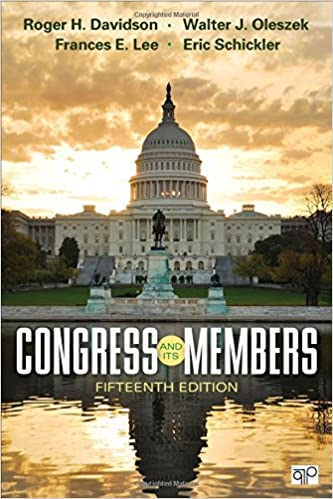
\includegraphics[width=0.9\linewidth]{congress.jpg}}
\end{wrapfigure}

I selected the fifteenth edition, but both older and newer editions will work. I picked the fifteenth edition only because it can be bought new on Amazon for \$15 and it's even less for a used copy! We'll also use all but two chapters of the book so you aren't paying for a bunch of extra material that we won't use. 

In addition to the textbook, I will also assign various new stories that serve as case studies of how Congress \textit{really} works. It's my hope that these articles will help to understand the ways in which the actual functioning of Congress has diverged from the founders intentions overtime. These case studies will be posted to iLearn and will be the basis of in-class activities and assignments. Don't neglect to read them!


\section*{Course Promises}

In this course, I will make the following promises to you. By the end of the semester, you will be able to:

\begin{enumerate}
	\item Explain how public policy is made in the U.S. 
	\item Describe the key factors that intervene with the passage of legislation.
	\item Identify the strategies members use to win elections and keep their approval high.
	\item Describe how Congress helps to keep other branches of government in check.
	\item Predict how individuals will behave if they are required to operate under a certain set of rules
\end{enumerate}


\section*{Course Expectations}

This course will only fulfill these promises if you promise the following in return:

\begin{enumerate}
	\item \textbf{To attend class.} I have designed this class for the readings and lectures to complement one another. As a result, attending lecture will be an essential component for your to develop a mastery of the course material. 
	\item \textbf{To read the assigned materials.} Similar to the lectures, the readings will provide additional details on each topic that may not be covered in lecture. They will also give you an opportunity to practice applying your knowledge of American government to understand real world decisions that have been made.
	\item \textbf{To be attentive and participate in class.} Participation does not only mean speaking aloud in class. Students should participate by actively following class discussions and engaging with lecture activities. 
	\item \textbf{To complete the required assignments in a timely fashion.} The assignments in this course are designed for you, and me, to measure your progress on meeting the course promises. Each assignment will give you practice at mastering these promises and I will give feedback to help guide you in your journey. Providing feedback is time consuming, however, so you will get the most useful feedback, and therefore the most use out of each assignment, only if you turn in your work on time.  
\end{enumerate}


\section*{Assignments and Evaluation}

Because writing is an essential component of nearly all career paths (and learning to write well is hard!) we will have several short writing assignments in the course. These assignments are designed to help you become a better writer, to get you to think more carefully about how governments work, to get you to think more carefully about how political decisions are made, and how to use evidence to support an argument. Below is a list of the writing assignments that we will complete in the course and their requirements. 

\begin{enumerate}
	\item \textbf{Google Documents Essay:} For your first assignment, you will answer the following question in \textbf{12pt font, 3 to 4 double-spaced pages}: \textit{``Why were the founders motivated to adopt a system of federalism in the U.S. and what were they hoping that this system would accomplish? How has this system complicated the ability of state governments and the federal government to make decisions? Finally, do you think that federalism is worth it or do you think that creates more problems than benefits? Why?"} \\ Good news, I will help you write this paper! You will use a Google Document that I have created for each of you to write this essay and I will be logging in to give you feedback and suggestions as you write. There is one caveat - I will match your level of effort. If you put a lot of work into your thinking and writing, I will give you more feedback and guidance.  {\color{red} This assignment is due on October 30th.} On that day I will restrict your ability to make any changes to your paper and will begin grading them. By working with you write your paper, I will be able to help you improve your writing \textit{before} you are graded on it and this will also allow me to encourage you think through your arguments, thus making you a better researcher and writer. This assignment will contribute to the 3rd, 5th, and 6th course promises. 
	\item \textbf{Midterm Essay:} This essay will be written in class and you will choose 1 prompt from a list of 3 different prompts. Before the exam, however, I will post a list of 6 essay prompts on iLearn and I will choose 3 of these prompts for the exam. You will need to answer the question in a \textbf{maximum of 2 pages.} \textbf{Please bring a Blue Book to use for the exam}. {\color{red} The midterm essay will be on November 6th.} This exam will require you to use your knowledge of the course material so far to support an argument. This assignment will contribute to the 5th and 6th course promises. 
	\item \textbf{Research Essay:} The final essay will be an original research paper of \textbf{a maximum of 5 pages double-spaced}. This assignment will be completed in stages that mimic how political scientists learn about the way that political events work, why politicians and governments do what they do. This project is an effort to teach you how to be a political scientist. This project will be completed in the following 3 stages:
		\begin{itemize}
			\item \underline{Project Proposal:} you will submit a project proposal that explains what question you will be researching and what you think the answer is in \textbf{50 words or less}. An essential aspect of any research project is identifying what puzzle you want to solve (the research question), as well as a prediction about the answer based on your knowledge of the topic (a hypothesis). {\color{red} This is due in-class on November 18th.}
			\item \underline{Project Outline:} In a \textbf{maximum of 1 double-spaced page}, you will create an outline of your paper. This outline should contain your research question, your argument, and how each paragraph will be used to support your argument. What evidence will you use? How will you convince your fellow political scientists that you are right?  {\color{red} Your project proposal will be submitted via iLearn on December 2nd.}
			\item \underline{Final Project:} Write your most convincing case for why your answer to your research question is the right one in a \textbf{maximum of 5 double-spaced pages}. If you have done the previous stages correctly, this will involve transforming your outline into a complete paper. {\color{red} The final paper will be submitted via iLearn on December 16th.}  
		\end{itemize} 
\end{enumerate}

In addition to these assignments, you will also be evaluated based on your participation in class activities. This involves being engaged during partner or group work, contributing to class discussions, and completing in-class participation assignments. You will also be asked to complete a short self-assessment of your participation in class at the end of the quarter. {\color{red} This assessment will be completed online and is due on December 16th.}  

These assignments will constitute your grade in the course and the weight of each of assignment are as follows:

\begin{center}
	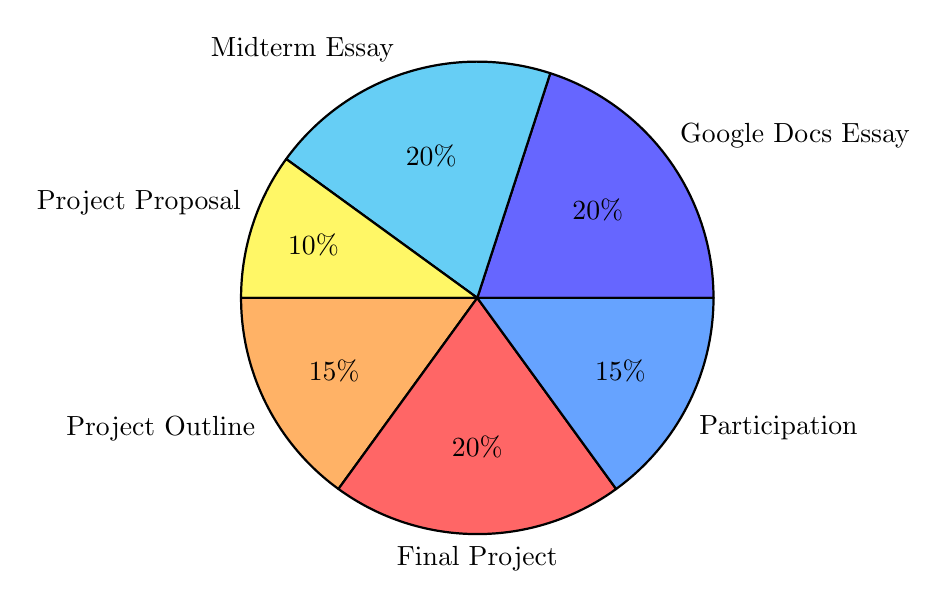
\begin{tikzpicture} 
		\pie{20/Google Docs Essay, 20/Midterm Essay, 10/Project Proposal, 15/Project Outline, 20/Final Project, 15/Participation}
	\end{tikzpicture}	
\end{center}

The letter grades will be assigned according to these percentages:

\begin{center}
	\begin{tabular}{ l l l l l l l l l l}
		\toprule
 		A+ & 97-100\% & B+ & 87-89\% & C+ & 77-79\% & D+ & 67-69\% & F & 0-59\% \\
		A & 93-96\% & B & 83-86\% & C & 73-76\% & D & 63-66\% \\
		A- & 90-92\% & B- & 80-82\% & C- & 70-72\% & D- & 60-62\% \\
		\bottomrule    
	\end{tabular}
\end{center}


\section*{Classroom Decorum and Academic Discourse}

For everyone to have the best possible learning experience, we will strive to create a classroom environment that supports respectful, critical inquiry through the free exchange of ideas. As part of learning, it is essential to discuss topics with individual who have different viewpoints than your own and the only way we can better understand one another is if we can carry on a collegial discussion of the topic. Remember, the goal is to become better critical thinkers. To do so we must learn to listen to others and articulate our views in respectful ways. As such, the following principles will guide our discussions:

\begin{itemize}
\item Treat every member of the class with respect, even if you disagree with their opinion;
\item Bring light, not heat;
\item Reasonable minds can differ on any number of perspectives, opinions, and conclusions;
\item Because constructive disagreement sharpens thinking, deepens understanding, and reveals novel insights, it is not just encouraged, it is expected;
\item No ideas are immune from scrutiny and debate;
\item You will not be graded on your opinions;
\item Arguments and evidence should be judged \emph{independently} of who offers such arguments and evidence. 
\end{itemize}

Additionally, to build a classroom environment that maximizes everyone's ability to master the course material please be mindful to not distract your fellow learners with your phone, tablet, or computer. It's perfectly fine if you would like to use these devices to take notes during class, but don't use them to distract yourself or your peers! Similarly, if you come late (or must leave early) please to enter/depart  the classroom in the least disruptive manner possible. This includes sitting near the door if you anticipate leaving early or taking a seat as near to the door as possible if you arrive late. 


\section*{Academic Honesty}

I expect that all work you produce for this course will be your own. If you plagiarize any material from outside sources for your written work or presentation in this course, or on the final exam, \textbf{it will result in a failure of the entire course.} There are no exceptions to this, and no second chances. Please refer to the university's \href{https://conduct.ucr.edu/policies/academic-integrity-policies-and-procedures}{Academic Integrity Polices \& Procedures} if you have questions about these standards. 


\section*{Special Accommodations}

If you need particular accommodations to help you succeed in mastering this course's material, please contact the \href{https://sdrc.ucr.edu}{Student Disability Resource Center} on campus in Costo Hall 125 to get a personalized accommodation plan.


\section*{Course Outline}

This syllabus is a working document. I reserve the right to make changes to the assigned readings (additions or deletions) or to the order of topics we cover as I deem necessary. Announcements regarding schedule changes will be made in class, in discussion sections, or on iLearn.

Also note that this schedule lists the topics of discussion for each class. To master the course material, you should finish each meeting's readings before we discuss them in class. This schedule also indicates which course promise(s) each class contributes to. They are listed as \textbf{CP} followed by the specific promise's number (listed above). 

\paragraph*{Tentative Schedule:}
\begin{center}
\begin{calendar}{8/31/2020}{16} % Semester starts on 1/11/2010 and last for 12
                    % weeks, including finals week
\setlength{\calboxdepth}{.3in}
\MWClass
% schedule
\caltexton{1}{\textbf{CP 1} \\ Course Introduction; Who are your Congressional representatives?}
\caltextnext{\textbf{CP 1} \\ Congress and Its Members Ch. 1: What exactly is Congress and what do members do?}
\caltextnext{\textbf{CP 1} \\ Congress and Its Members Ch. 2 S. 1 \& 2: Why a ``Congress?"}
\caltextnext{\textbf{CP 1 \& 4} \\ Congress and Its Members Ch. 2 S. 3-5: How has Congress changed over time?}
\caltextnext{\textbf{CP 3} \\ Congress and Its Members Ch. 3 S. 1 \& 2: You gotta know the rules before you play (Campaign and election procedures).}
\caltextnext{\textbf{CP 1} \\ Congress and Its Members Ch. 3 S. 3-5: Entering the electoral race.}
\caltextnext{\textbf{CP 1 \& 3} \\  {\color{red} Problem Set 1 Due via iLearn} \\ Congress and Its Members Ch. 4 S. 1-4: How to win!}
\caltextnext{\textbf{CP 1 \& 3} \\ Congress and Its Members Ch. 4 S. 5-8: What candidates need to know about voters.}
\caltextnext{\textbf{CP 1, 2, \& 3} \\ Congress and Its Members Ch. 5 S. 1 \& 2: What do legislators really care about?}
\caltextnext{\textbf{CP 1, 2, \& 3} \\ Congress and Its Members Ch. 5 S. 3-5: You better be a people person and love traveling!}
\caltextnext{\textbf{CP 1 \& 2} \\  {\color{red} Project Proposal Due In-Class} \\ Congress and Its Members Ch. 6 S. 1-4: Getting to know the bosses (leadership positions in Congress).}
\caltextnext{\textbf{CP 1} \\ Congress and Its Members Ch. 6 S. 5-9: Supporting your team and joining clubs (Party committees and caucuses).}
\caltextnext{\textbf{CP 1 \& 3} \\ Congress and Its Members Ch. 7 S. 1-4: Learn how things get done around here (committees).}
\caltextnext{\textbf{CP 1 \& 2} \\ {\color{red} Problem Set 2 Due via iLearn} \\ Congress and Its Members Ch. 7 S. 5-9: What happens after a bill gets introduced?}
\caltextnext{\textbf{CP 1 \& 2} \\ Congress and Its Members Ch. 8 S. 1-4: The House has a lot of rules.}
\caltextnext{\textbf{CP 1 \& 2} \\ Congress and Its Members Ch. 8 S. 5-8: So does the Senate...}
\caltextnext{\textbf{CP 1} \\ Congress and Its Members Ch. 9 S. 1-2: What exactly do you do in Congress?}
\caltextnext{\textbf{CP 1 \& 3} \\ Congress and Its Members Ch. 9 S. 3-5: How much freedom do members have in Congress?}
\caltextnext{\textbf{CP 1} \\ Congress and Its Members Ch. 10 S. 1-2: Can the president really affect legislation?}
\caltextnext{\textbf{CP 1, 3, \& 4} \\ Congress and Its Members Ch. 10 S. 3-5: How the president can stifle all your hard work.}
\caltextnext{\textbf{CP 1 \& 2} \\ {\color{red} Midterm}}
\caltextnext{\textbf{CP 1 \& 4} \\ Congress and Its Members Ch. 11 S. 1: Keepin' an eye on the bureaucracy}
\caltextnext{\textbf{CP 1 \& 4} \\ {\color{red} Project Outline Due via iLearn} \\ Congress and Its Members Ch. 11 S. 2-3: How can Congress exercise control of the bureaucracy?}
\caltextnext{\textbf{CP 1 \& 2} \\ {\color{red} Problem Set 3 Due via iLearn} \\ Congress and Its Members Ch. 12: How does Congress interact with the Supreme Court?}
\caltextnext{\textbf{CP 1 \& 2} \\ Congress and Its Members Ch. 13 S. 1-2: Where do organized interests come in?}
\caltextnext{\textbf{CP 1 \& 2} \\ Congress and Its Members Ch. 13 S. 3-5: Does money matter more than constituents?}
\caltextnext{\textbf{CP 1, 2, \& 4} \\ }
\caltextnext{{\color{red} Final Project Due on iLearn (CP 5 \& 6) \\ Participation Self-assessment Due}}
% ... and so on

% Holidays
\Holiday{9/7/2020}{\textbf{Labor Day - No Class :(}}
\Holiday{11/23/2020}{\textbf{Thanksgiving Break! - No Class :(}}
\Holiday{11/24/2020}{\textbf{Thanksgiving Break! - No Class :(}}
\Holiday{11/25/2020}{\textbf{Thanksgiving Break! - No Class :(}}
\Holiday{11/26/2020}{\textbf{Thanksgiving Break! - No Class :(}}
\Holiday{11/27/2020}{\textbf{Thanksgiving Break! - No Class :(}}
\Holiday{11/28/2020}{\textbf{Thanksgiving Break! - No Class :(}}
% ... and so on

\options{4/26/2010}{\noclassday} % finals week
\options{4/27/2010}{\noclassday} % finals week
\options{4/28/2010}{\noclassday} % finals week
\options{4/29/2010}{\noclassday} % finals week
\options{4/30/2010}{\noclassday} % finals week
\caltext{4/27/2010}{\textbf{Final Exam}}
\end{calendar}
\end{center}

\end{document}